\documentclass[usenames,dvipsnames,8pt,aspectratio=169]{beamer}
\usepackage{amsmath,amsfonts,amssymb}
\usepackage{mathtools}
\usepackage{etex} %for Windows
\usepackage[utf8]{inputenc}
\usepackage[english, russian]{babel} 

%\usepackage{microtype}			% Better interword spacing and additional kerning.
\usepackage{ellipsis}			% Adjusted space with \dots between two words.
\usepackage{graphicx}
\usepackage{pstricks}

\usepackage{xcolor}


\usepackage{changepage}

\usepackage{algorithm}
\usepackage{algpseudocode}
%\usepackage[]{algorithm2e}
%\usepackage{algorithmic}

%\usepackage{tcolorbox}


\usepackage{tikz}
\usetikzlibrary{tikzmark,calc}
\usetikzlibrary{positioning, backgrounds}
\usetikzlibrary{arrows, chains, matrix, scopes, patterns, shapes, fit}
\usetikzlibrary{mindmap,trees,shadows}
\usetikzlibrary{decorations.pathreplacing}

\usepackage{pgfplots}

\pgfmathdeclarefunction{gauss}{2}{%
	\pgfmathparse{1/(#2*sqrt(2*pi))*exp(-((x-#1)^2)/(2*#2^2))}%
}


\tikzset{
	invisible/.style={opacity=0},
	visible on/.style={alt={#1{}{invisible}}},
	alt/.code args={<#1>#2#3}{%
		\alt<#1>{\pgfkeysalso{#2}}{\pgfkeysalso{#3}} % \pgfkeysalso doesn't change the path
	},
}

\newcommand\strikeout[2][]{%
	\begin{tabular}[b]{@{}c@{}} 
		\makebox(0,0)[cb]{{#1}} \\[-0.2\normalbaselineskip]
		\rlap{\color{Orange}\rule[0.5ex]{\widthof{#2}}{1.5pt}}#2
\end{tabular}}

\newcommand\Fontvi{\fontsize{11}{13.2}\selectfont}

\usepackage{listings} % for C++ code

\usepackage{braket}
%\usepackage[braket, qm]{qcircuit}



\usepackage[T1]{fontenc}
%\usepackage[sfdefault,scaled=.85]{FiraSans}
%\usepackage{newtxsf}
%\usepackage[nomap]{FiraMono}



%\renewtheorem{theorem}{Теорема}
%\renewtheorem{lemma}{Лемма}
%\renewtheorem{definition}{Определение}
%\renewtheorem{corollary}{Следствие}
%\renewtheorem{fact}{Факт}

\usefonttheme[onlymath]{serif}
\renewcommand\sfdefault{cmbr}

\renewcommand{\bfdefault}{sb}

\definecolor{CharCoalDark}{RGB}{13, 16, 19}
\definecolor{Orange}{RGB}{255, 165,0}
\definecolor{DarkOrange}{RGB}{255, 165,0}
\definecolor{LightSalmon}{RGB}{255, 160, 122}
\definecolor{LeafGreen}{RGB}{34, 139,  34}
\definecolor{Coral}{RGB}{255, 127, 80}
\definecolor{DarkTurquoise}{RGB}{0, 206, 209}

\definecolor{darkslateblue}{RGB}{72,61,139}

%\newtheorem{defRus}{Определение}
%\newtheorem{thmRus}{Теорема}
%s\newtheorem{corRus}{Следствие}

\def\darktheme{}
\ifdefined\darktheme
	\setbeamercolor{background canvas}{bg=CharCoalDark}
	\setbeamerfont{title}{series=\bfseries}
	\setbeamercolor{title}{fg=Orange}
	\setbeamercolor{section in toc}{fg=white}
	\setbeamercolor{frametitle}{fg=Orange}
	\setbeamercolor{normal text}{fg=white}
	%\setbeamercolor{normal text}{fontsize=12pt}
	\setbeamercolor{itemize item}{fg=Orange}
	\setbeamercolor{itemize item item}{fg=Orange}
	\setbeamercolor{enumerate item}{fg=Orange}
	\setbeamercolor{block title}{bg=DarkOrange,fg=white}
	\setbeamerfont{block title}{series=\bfseries}
	
	\setbeamertemplate{itemize item}[circle]
	%\setbeamertemplate{itemize subitem}[$\checkmark$]
	\setbeamertemplate{itemize subitem}{\color{Orange}\Large$\textbullet$}
	\setbeamertemplate{itemize subitem}{\color{Orange} \tiny $\blacksquare$}
\else
	\setbeamercolor{background canvas}{bg=white}
	\setbeamerfont{title}{series=\bfseries}
	\setbeamercolor{title}{fg=darkslateblue}
	\setbeamercolor{section in toc}{fg=black}
	\setbeamercolor{frametitle}{fg=darkslateblue}
	\setbeamercolor{normal text}{fg=black}
	%\setbeamercolor{normal text}{fontsize=9pt}
	\setbeamercolor{itemize item}{fg=darkslateblue}
	\setbeamercolor{itemize item item}{fg=darkslateblue}
	\setbeamercolor{enumerate item}{fg=darkslateblue}
	\setbeamercolor{block title}{bg=darkslateblue,fg=white}
	\setbeamerfont{block title}{series=\bfseries}
	
	\setbeamertemplate{itemize item}[circle]
	%\setbeamertemplate{itemize subitem}[$\checkmark$]
	\setbeamertemplate{itemize subitem}{\color{blue}\Large$\textbullet$}
	\setbeamertemplate{itemize subitem}{\color{blue} \tiny $\blacksquare$}

\fi

% footnote without a marker
\newcommand\blfootnote[1]{%
	\begingroup
	\renewcommand\footnoterule{}
	\renewcommand\thefootnote{}\footnote{#1}%
	\addtocounter{footnote}{-1}%
	\endgroup
}

\newcommand*{\Scale}[2][4]{\scalebox{#1}{\ensuremath{#2}}}%

\newcommand\Item[1][]{%
	\ifx\relax#1\relax  \item \else \item[#1] \fi
	\abovedisplayskip=0pt\abovedisplayshortskip=0pt~\vspace*{-\baselineskip}}

\pgfdeclareradialshading{ring}{\pgfpoint{0cm}{0cm}}%
{rgb(0cm)=(1,1,1);
	rgb(0.7cm)=(1,1,1);
	rgb(0.719cm)=(1,1,1);
	rgb(0.72cm)=(0.975,0,0);
	rgb(0.9cm)=(1,1,1)}

\usepackage[absolute,overlay]{textpos} %to clip to a corner
\newcommand\FrameText[1]{%
	\begin{textblock*}{\paperwidth}(\textwidth-35pt, 10 pt)
		\raggedright #1\hspace{.5em}
\end{textblock*}}

\makeatletter
\let\save@measuring@true\measuring@true
\def\measuring@true{%
	\save@measuring@true
	\def\beamer@sortzero##1{\beamer@ifnextcharospec{\beamer@sortzeroread{##1}}{}}%
	\def\beamer@sortzeroread##1<##2>{}%
	\def\beamer@finalnospec{}%
}
\makeatother

\AtBeginSection[]
{
	\begin{frame}<beamer>
		\frametitle{Outline}
		\tableofcontents[currentsection]
	\end{frame}
}


\title{Лекция №1 \\[10pt]
		Часть 1. О курсе}

\date{ Елена Киршанова \\  \textbf{Курс ``Основы криптографии''} \\  }


\setbeamertemplate{navigation symbols}{} %removes navigation

% proper highlightling of a code-snippet
\lstset{language=C++,
	keywordstyle=\color{magenta},
	stringstyle=\color{Goldenrod},
	commentstyle=\color{gray},
	breaklines=false,
	%morecomment=[l][\color{magenta}]{\#}
}

%\setlength{\parskip}{8pt}
% ==================================================================
% Definitions for this paper
% ==================================================================
\mathchardef\hyphen="2D

\usepackage{multirow}
\usepackage{multicol} % For multiple coloumn environments
%\usepackage{stmaryrd} % For set brackets
% \setlength{\columnsep}{15pt} % Defining the coloumn seperation
% \setlength{\columnseprule}{1pt} % Place a line between coloumns
% \newcommand{\tab}{\hspace*{2em}}

%subscripts

\newcommand*\SmallTextScript[2]{{\mathchoice{\displaystyle #2}
		{\textstyle #2}%dito
		{\scalebox{#1}{\ensuremath{\scriptstyle #2}}}%
		{\scalebox{#1}{\ensuremath{\scriptscriptstyle #2}}}%
}}


% ADVERSARIES AND SUCH
\newcommand*{\poly}{\ensuremath{\mathrm{poly}}}
\newcommand*{\eps}{\ensuremath{\varepsilon}}
\newcommand*{\alg}{\ensuremath{\mathcal{A}}}

% GROUPS/DISTRIBUTIONS/SETS/LISTS
\newcommand{\N}{{{\mathbb N}}}
\newcommand{\Z}{{{\mathbb Z}}}
\newcommand*{\IZ}{\ensuremath{\mathbb{Z}}}
\newcommand*{\IN}{\ensuremath{\mathbb{N}}}
\newcommand*{\IQ}{\ensuremath{\mathbb{Q}}}
\newcommand{\R}{{{\mathbb R}}}
\newcommand*{\IR}{{{\mathbb R}}}
\newcommand{\Zp}{\ints_p} % Integers modulo p
\newcommand{\Zq}{\ints_q} % Integers modulo q
\newcommand{\Zn}{\ints_N} % Integers modulo N
\newcommand{\F}{\ensuremath{\mathbb{F}}}
\newcommand{\CC}{\ensuremath{\mathbb{C}}}

\newcommand{\GF}{\ensuremath{\mathbb{F}_2}}
\newcommand{\GFn}{\ensuremath{\mathbb{F}^n_2}}

%%% ALGORITHMS/PROCEDURES %%%
\newcommand{\Dec}{\textsf{Dec}}
\newcommand{\Enc}{\textsf{Enc}}
\newcommand{\KeyGen}{\textsf{KeyGen}}
\newcommand{\Gen}{\textsf{Gen}}
\newcommand{\sk}{\textsf{sk}}
\newcommand{\pk}{\textsf{pk}}
\newcommand{\vk}{\textsf{vk}}
\newcommand{\mesS}{\ensuremath{\mathcal{M}}}
\newcommand{\keyS}{\ensuremath{\mathcal{K}}}
\newcommand{\cipS}{\ensuremath{\mathcal{C}}}
\newcommand{\tagS}{\ensuremath{\mathcal{T}}}
\newcommand{\mactag}{\textsf{tag}}
\newcommand{\Hash}{\ensuremath{\mathcal{H}}}
\newcommand{\EID}{\ensuremath{\mathtt{EphID}}}


\newcommand{\adv}{\ensuremath{\mathcal{A}}}

\newcommand{\LWE}{\mathsf{LWE}}
\newcommand{\DCP}{\mathsf{DCP}}
\newcommand{\EDCP}{\mathsf{EDCP}}
\newcommand{\UEDCP}{\mathsf{U \text{-} EDCP}}
\newcommand{\GEDCP}{\mathsf{G \text{-} EDCP}}



%% Landau and proba
\newcommand{\bigO}{\mathcal{O}}
\newcommand*{\OLandau}{\bigO}
\newcommand*{\WLandau}{\Omega}
\newcommand*{\xOLandau}{\widetilde{\OLandau}}
\newcommand*{\xWLandau}{\widetilde{\WLandau}}
\newcommand*{\TLandau}{\Theta}
\newcommand*{\xTLandau}{\widetilde{\TLandau}}
\newcommand{\smallo}{o} %technically, an omicron
\newcommand{\wLandau}{\omega}
\newcommand{\negl}{\mathrm{negl}}
\newcommand*\PROB\Pr 
\DeclareMathOperator*{\EXPECT}{\mathbb{E}}
\DeclareMathOperator*{\VARIANCE}{\mathbb{V}}
\DeclareMathOperator*{\LOGBIAS}{\mathbb{LB}}

\newcommand{\supp}{\ensuremath{\mathsf{sup}}}
\newcommand{\Distr}{\ensuremath{\mathcal{D}}}

% Lattices

% \newcommand{\coset}{\Lambda} % Lambda Lattice
% \newcommand{\cosetPerp}{\Lambda^{\bot}} % Lambda_Perp Lattice
% \newcommand{\gadget}{\textbf{G}} %Gaget matrix
% \newcommand{\mes}{\textbf{m}} %message vector
% \newcommand{\AMat}{\textbf{A}} %A matrices
% \newcommand{\BMat}{\textbf{B}} %B matrices
% \newcommand{\RMat}{\textbf{R}} %R matrices
% \newcommand{\HMat}{\textbf{H}} %H matrices
% \newcommand{\XMat}{\textbf{X}} %H matrices
% \newcommand{\mbar}{\bar{m}} %mBar dimension
% % \newcommand{\gauss}{\mathcal{D}} % gaussian distribution
% \newcommand{\Id}{\textbf{I}} % Identity matrix
% \newcommand{\er}{\textbf{e}} % gaussian distr. vectors
% % \newcommand{\cipher}{\textit{c}} % ciphertext
% \newcommand{\Olwe}{\mathcal{O}_{\textsf{LWE}}} %LWE oracle
% \newcommand{\OSample}{\mathcal{O}_{Sample}} %LWE oracle
% \newcommand{\SigmaB}{\boldsymbol{\Sigma}} %semi-deifinite matrix Sigma%
% % \newcommand{\mods}{\text{ mod}}


%Vectors and Matrices

\newcommand{\AMat}{\mathbf{A}} %A matrices
\newcommand{\BMat}{\mathbf{B}} %B matrices
\newcommand{\DMat}{\mathbf{D}} %Diagonal


\newcommand{\HMat}{\ensuremath{\mathbf{H}}}
\newcommand{\QMat}{\ensuremath{\mathbf{Q}}}
\newcommand{\Id}{\ensuremath{\mathbf{I}}}
\newcommand{\ZeroM}{\textbf{0}} % Zero matrix

\newcommand{\avec}{\ensuremath{\mathbf{a}}}
\newcommand{\bvec}{\ensuremath{\mathbf{b}}}
\newcommand{\cvec}{\ensuremath{\mathbf{c}}}
\newcommand{\evec}{\ensuremath{\mathbf{e}}}
\newcommand{\rvec}{\ensuremath{\mathbf{r}}}
\newcommand{\svec}{\ensuremath{\mathbf{s}}}
\newcommand{\tvec}{\ensuremath{\mathbf{t}}}
\newcommand{\vvec}{\ensuremath{\mathbf{v}}}
\newcommand{\zvec}{\ensuremath{\mathbf{z}}}
\newcommand{\xvec}{\ensuremath{\mathbf{x}}}
\newcommand{\yvec}{\ensuremath{\mathbf{y}}}
\newcommand{\uvec}{\ensuremath{\mathbf{u}}}
\newcommand{\zerovec}{\ensuremath{\mathbf{0}}}

\newcommand{\nth}{^{\mathrm{th}}}
\newcommand{\nd}{^{\mathrm{nd}}}

\newcommand{\RepMMT}{\ensuremath{\mathcal{R}_{\protect\SmallTextScript{0.70}{\texttt{MMT}}}}}
\newcommand{\RepBJMM}{\ensuremath{\mathcal{R}_{\protect\SmallTextScript{0.70}{\texttt{BJMM}}}}}
\newcommand{\XOR}{\ensuremath{\mathtt{3XOR}}}


% % % % % \newcommand{\mb}[1]{\mathbf{#1}} % does not compile otherwise
%%% Removed by Gotti; this is just asking to screw up with packages that (properly) define \mb (mathbold)

% \newcommand{\bL}{\|\bvec_1\|} % b1 length that appears way too often
% \newcommand{\dL}{\|\dvec_1\|} % b1 length that appears way too oftend

%Norms and Scalar products

\newcommand*\abs[1]{\left\lvert#1\right\rvert}
\newcommand*\norm[1]{\left\lVert#1\right\rVert}
\newcommand*\normalabs[1]{\lvert#1\rvert} 
\newcommand*\normalnorm[1]{\lVert#1\rVert}
\newcommand*\bignorm[1]{\bigl\lVert#1\bigr\rVert}
\newcommand*\bigabs[1]{\bigl\lvert#1\bigr\rvert}
\newcommand*\Bigabs[1]{\Bigl\lvert#1\Bigr\rvert}
\newcommand*{\ScProd}[2]{\ensuremath{\langle#1\mathbin{,}#2\rangle}} %Scalar Product
% \newcommand*{\ScProd}[2]{\ensuremath{\langle#1 \:{,}\:#2\rangle}} %Scalar Product
\newcommand*{\bigScProd}[2]{\ensuremath{\bigl\langle#1\mathbin{,}#2\bigr\rangle}} %Scalar Product
\newcommand*{\BigScProd}[2]{\ensuremath{\Bigl\langle#1\mathbin{,}#2\Bigr\rangle}} %Scalar Product
\newcommand{\dist}{\ensuremath{\text{dist}}}


%Some other math operators

\DeclareMathOperator{\Span}{Span} %span of vectors
\DeclareMathOperator{\vol}{\mathrm{vol}} %volume
\DeclareMathOperator{\LW}{LambertW} %Lambert W function
\DeclareMathOperator{\SD}{SD}
\DeclareMathOperator{\gradient}{grad}
\DeclareMathOperator{\TRACE}{Tr}
\newcommand*{\dDR}{\mathrm{d}} %de-Rham-Differential (the d in dx, dy, dz and so on)


%Lists
\renewcommand{\L}{\ensuremath{\mathcal{L}}}

\renewcommand{\P}{\ensuremath{\mathcal{P}}}

\newcommand*{\Lout}{\ensuremath{\L_{\mkern-0.5mu\protect\SmallTextScript{0.85}{\textup{out}}}}}
\newcommand*{\Sout}{\ensuremath{S_{\mkern-0.5mu\protect\SmallTextScript{0.85}{\textup{out}}}}}
\newcommand{\wt}{\ensuremath{\mathit{wt}}}


\newcommand*{\softO}{\widetilde{\bigO}}

\newcommand{\const}{\mathsf{c}} 


\newcommand{\transpose}{\mkern0.7mu^{\mathsf{ t}}}

%proper overline reduced by 1.5mu
\newcommand{\overbar}[1]{\mkern 1.5mu\overline{\mkern-1.5mu#1\mkern-1.5mu}\mkern 1.5mu}

\DeclareMathOperator{\erf}{erf} %error function
\DeclareMathOperator{\erfc}{erfc} %complementary error function
\newcommand{\Er}{\ensuremath{\mathrm{Er}}} %complementary error function


% LATTICES

\newcommand{\Lat}{\ensuremath{\mathcal{L}}}
\newcommand*{\Sphere}[1]{\ensuremath{\mathsf{S}^{#1}}}
%\DeclareMathOperator{\Conf}{Conf}
\newcommand{\Conf}{\mathcal{C}}

%Thick line for table
\setlength{\doublerulesep}{0pt}
\newcommand{\thickline}{\hline\hline\hline}


%circled text
\newcommand*\circled[1]{\tikz[baseline=(char.base)]{
    \node[shape=circle,draw,inner sep=0.3 pt] (char) {\scriptsize #1};}}


%Fix Algorithmicx package
\def\NoNumber#1{{\def\alglinenumber##1{}\State #1}\addtocounter{ALG@line}{-1}}

%For comments
\newcommand{\GColor}{ForestGreen}  %Damiens' color
\newcommand{\EColor}{MidnightBlue} %Elena's color

\newcommand*{\E}[1]{{\color{\EColor} #1} } 
\newcommand*{\G}[1]{{\color{\GColor} #1} } 

%Proper limit with the subscript underneath
% \newcommand{\Lim}[1]{\raisebox{0.5ex}{\scalebox{0.8}{$\displaystyle \lim_{#1}\;$}}}


%TIKZ dense dotted pattern

\pgfdeclarepatternformonly{my dots}{\pgfqpoint{-1pt}{-1pt}}{\pgfqpoint{2.0pt}{2.0pt}}{\pgfqpoint{2pt}{2pt}}%
{
	\pgfpathcircle{\pgfqpoint{0pt}{0pt}}{.35pt}
	\pgfpathcircle{\pgfqpoint{1pt}{1pt}}{.35pt}
	\pgfusepath{fill}
}


\tikzset{
	master/.style={
		execute at end picture={
			\coordinate (lower right) at (current bounding box.south east);
			\coordinate (upper left) at (current bounding box.north west);
		}
	},
	slave/.style={
		execute at end picture={
			\pgfresetboundingbox
			\path  (lower right)rectangle (upper left) ;
		}
	}
} %all defs
\begin{document}
	
\begin{frame}
	\titlepage
\end{frame}


\begin{frame}{Админ}
\Large
\begin{itemize}
	\itemsep 12pt
	\item Встречаемся в Webinar по вторникам в 17:10 по Калининграду
	\item Лабораторные принимаются после лекций
	\item Страница курса  \\
	\url{https://crypto-kantiana.com/elena.kirshanova/teaching/info_sec\_2022.html}
	\item Для прохождения курса: сдача всех лабораторных + тест в день зачёта
\end{itemize}
\end{frame}


\begin{frame}{Лабораторные работы}
\Large
\begin{itemize}
	\itemsep 12pt
	\item После каждой лекции будет опубликовано задание к лабораторной работе, например\\
	\url{https://crypto-kantiana.com/elena.kirshanova/teaching/info_sec2022/Lab1.txt}
	\item Реализовывать алгоритмы можно (и рекомендуется) с помощью библиотек OpenSSL, либо crypto++ (обе С++)
	\item Лабораторные работы выполняются индивидуально
\end{itemize}
\end{frame}

\begin{frame}{Структура и план курса}

\Large
{\color{Orange} I. Симметрическая криптография} \\[10pt]
\begin{itemize}
	\item 11/10 Псевдослучайные генераторы
	\item 18/10 Блок-шифры
	\item 25/10 Хэш-функции. Коды аутентификации сообщений 
\end{itemize}

\vspace{20pt}
{\color{Orange} II. Асимметрическая криптография}

\begin{itemize}
	\item 1/11 Обмен ключами
	\item 8/11 Цифровые подписи
\end{itemize}

\end{frame}

\begin{frame}{Чего не будет}

\Large

Мы {\color{Orange} не} будем говорить о

\begin{itemize}
	\itemsep 8pt
	\item блокчейнах
	\item программировании / реверс инжиниринге
	\item хакерстве
	\item квантовой и пост-квантовой криптографии
\end{itemize}

\end{frame}

\begin{frame}{Литература}
\Large
\begin{columns}[T]
	\begin{column}{0.5\textwidth}
		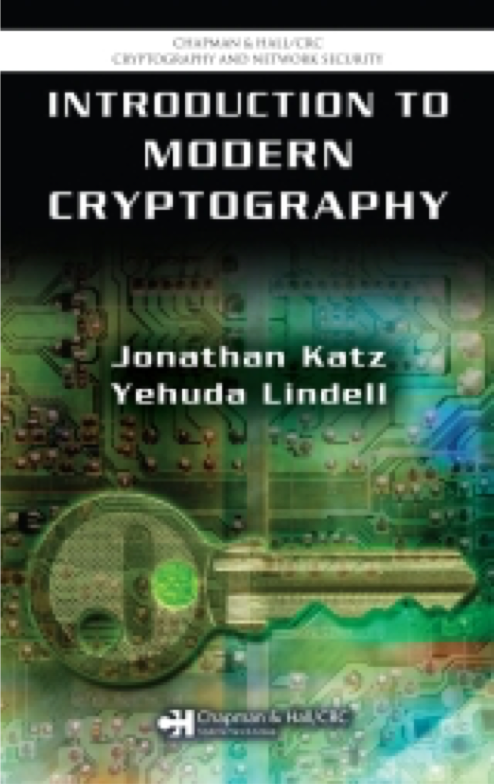
\includegraphics[scale=0.25]{katz_lindel_book}
	\end{column}
	\begin{column}{0.55\textwidth}
	\vspace{40pt}
	A Graduate Course in Applied Cryptography \\[5pt]
	Dan Boneh, Victor Shoup \\[5pt]
	\url{https://toc.cryptobook.us/book.pdf}
	\end{column}
\end{columns}

\end{frame}

\begin{frame}{Комментарии}

\Large
\begin{itemize}
	\itemsep 8pt
	\item Подразумеваем знания элементарных алгоритмов, тер. вера, линейной алгебры
	\item Будет много англоязычных слов!
	\item  Опечатки неизбежны
	\item Комментарии/замечания/пожелания/недовольства можно отправить по почте
	\[
	\text{elenakirshanova [at] gmail [dot] com}
	\]
\end{itemize}

\end{frame}


\begin{frame}
Часть II \\ [10pt]
\begin{LARGE}
	
	\color{Orange}
	\Huge Принципы криптографии \\
	
\end{LARGE}
\end{frame}

\begin{frame}{Определения I.}
\Large 
Принятая модель вычислений -- машина Тьюринга \\
\begin{block}{Полиномиальное время}
	Алгоритм $\alg$ работает за \emph{полиномиальное время}, если, получая на вход данные размера  $n$ бит,  $\alg$ терминирует за время $\bigO(n^k)$ для константы $k$.
\end{block}
\vspace{10pt}
Примеры: 
\begin{itemize}
	\LARGE
	\item умножение двух $n$-битных чисел: $\bigO(n \log n)$ -- полиномиальное время
	\item факторизация $n$-битного числа: $\exp(\bigO(n^{1/3}\cdot (\log n)^{2/3})$ -- субэкспоненциальное время
\end{itemize}
\vspace{10pt}
\Large

%\begin{block}{Вероятностное полиномиальное время (ppt)}
Алгоритм $\alg$ называется \emph{вероятностным полиномиальным} (ppt), \\ если он работает за полиномиальное время и использует \\ случайные биты.
%\end{block} 

\end{frame}


\begin{frame} {Определения II.}
\Large
\begin{block}{Пренебрежимо малая функция}
Функция $f: \N \rightarrow \R$ \emph{пренебрежимо мала} (negl), если для всех многочленов $p$ существует $N \in \N$, такое что для любого $n \geq N$
\[
f(n) < \frac{1}{p(n)}.
\]
\end{block}

\vspace{10pt}
Примеры: 
\begin{itemize}
\LARGE
\item negl:
\[
\frac{1}{2^n}, \; \frac{1}{2^{\sqrt{n}}}, \;  \frac{1}{2^{\log^2(n)}}
\]
\item non-negl:
\[
\frac{1}{\log n}, \;  \frac{1}{n^2}, \;  \frac{1}{2^{\bigO(\log n)}} 
\]
\end{itemize}
\end{frame}

\begin{frame}{Формальное описание шифра}
\Large
\begin{block}{Шифр-схема $\Pi=(\KeyGen, \Enc, \Dec)$}
включает в себя \emph{ppt} алгоритмы {\color{Orange} $\KeyGen, \Enc, \Dec$ } и множества
\begin{align*}
\keyS &- \text{множество ключей} \\
\mesS &- \text{множество открытых текстов}\\
\cipS &- \text{множество шифр-текстов}
\end{align*}
такими, что для
\begin{align*}
k &\leftarrow \KeyGen(1^\lambda) \\
c &\leftarrow \Enc(k, m) \\
m' & = \Dec(k, c) \\
\end{align*}
схема {\color{Orange}корректна}:
$
\Dec(k, \Enc(k, m)) == m \quad \forall k \in \keyS, m \in \mesS
$

%для элемента $m$ из пространства открытых текстов $\{\mesS_\lambda\}$ задана\\ функция длины, $\abs{m}$

\end{block}

\end{frame}

\begin{frame}{Шифр-схема (свойства)}
\Large
Формально: множества $\keyS, \mesS, \cipS$ зависят от {\color{Orange}пар-ра безопасности} $\lambda$.  \\[10pt]
%\itemsep 25pt
{Параметризация} шифр-схемы $\Param(\lambda)$ -- ppt алгоритм, принимающий на вход пар-р безопасности $\lambda$, и выдающий битовую строку $\Lambda = \poly(\lambda)$, задающую параметры шифр-схемы. \\[10pt]
Пример: Для криптографической хэш-функции SHA-256 с $\lambda=128$, $\Param(\lambda)$ выдаст 		
\[
\keyS_{128} =  \{0,1\}^{512} \qquad  \mesS_{128} =  \cipS_{128} = \{0,1\}^{256}  
\]

%\item Шифр-схема называется \emph{детерминированной}, если функция \\ шифрования $\Enc()$ -- детерминирована
\end{frame}

\begin{frame}{Основные принципы современной криптографии}
\LARGE
Принцип Керкгоффса (Kerckhoffs’ principle)\footnote{ Auguste Kerckhoffs, «La Cryptographie Militaire», 1883}: \\[10pt]

\texttt{ Криптосистема должна оставаться безопасной, если злоумышленнику известно всё, кроме секретного ключа} \\[30pt]


Алгоритмы $\Enc, \Dec, \Param$ являются открытыми и подлежат \\ открытым научным исследованиям

\end{frame}

\begin{frame}
Часть III \\ [10pt]
\begin{LARGE}
	
	\color{Orange}
	\Huge Абсолютная криптографическая стойкость. \\ Одноразовый блокнот\\
	
\end{LARGE}
\end{frame}

\begin{frame}{Шифр Шеннона (Shannon's cipher)}
\Large
Положим $\keyS, \mesS, \cipS$ -- множества ключей, открытых текстов, шифр-текстов 
\begin{block}{Шифр Шеннона --}
	это тройка функций $\KeyGen, \Enc, \Dec$:
	\begin{align*}
	\Enc: \keyS \times \mesS & \rightarrow \cipS \\
	\Enc(k, m)  &= c  \\[10pt]
	\Dec: \keyS \times \cipS & \rightarrow \mesS \\
	\Dec(k, c) &= m,
	\end{align*}
	для которых выполняется 
	\[
	\Dec(k, \Enc(k,m)) == m \qquad \forall k \leftarrow \KeyGen, m \in \mesS 
	\]
\end{block}
\end{frame}

\begin{frame}{Абсолютная криптографическая стойкость (perfect secrecy)}
\Large
\begin{itemize}
\itemsep 5pt
\item На каждом из этих множеств зададим распределение:  \\ $\Pr[M = m]$ -- вероятность выбора $m \in \mesS$.
\item Аналогично для $K \in \keyS, C \in \cipS$.
\end{itemize}

\begin{block}{Абсолютная криптографическая стойкость}
Шифр-схема $\Pi = (\KeyGen, \Enc, \Dec)$ обладает \emph{абсолютной криптографической стойкостью}, если для любого распределения над $\mesS$
\[
\Pr \left[ M= m | C = c\right] = \Pr\left[M = m\right] \quad \forall m \in \mesS, c \in \cipS.
\]
\end{block}
\textbf{Интуиция:} шифр-текст $c$ не содержит никакой информации об \\ открытом тексте $m$.
%	Equivalent definition:
%	\[
%		\Pr\left[\Enc(k, m_0) = c\right] = \Pr\left[\Enc(k, m_1) = c\right] \quad \forall m_0, m_1 \in \mesS, c \in \cipS.
%	\]
\end{frame}


\begin{frame}{Эквивалентные определения}
\Large
Шифр-схема $\Pi = (\Enc, \Dec)$ определена над $\keyS, \mesS, \cipS$ \\

\begin{enumerate}
	\itemsep 10pt
\item  Шифр-текст не зависит от открытого текста: 
\[
\Pr[C = c \; |\; M =m  ] = \Pr[C = c] \qquad \forall m \in \mesS, c \in \cipS.
\]

\item Шифр-тексты не отличимы друг от друга:  для любых $m_0, m_1 \in \mesS$ выполняется
\[
\Pr[C = c \; | \; M = m_0] = \Pr[C = c \; | \; M = m_1]
\]
\end{enumerate}
\end{frame}

\begin{frame}{Одноразовый блокнот (One-time pad) или шифр Вернама }
\LARGE
\vspace{-40pt}
\begin{block}{Одноразовый блокнот}
Положим $\mesS, \keyS, \cipS = \{0,1\}^n$.
\begin{itemize}
\item $\KeyGen(1^{\lambda}): k \leftarrow \{0,1\}^n$ \\[10pt]
\item $\Enc(k, m \in \{0,1\}^n): c = k \oplus m$ \\[10pt]
\item $\Dec(k, c \in \{0,1\}^n): m = k \oplus c$ \\[10pt]
\end{itemize}
\end{block}

{\color{Orange} Теорема.}
Одноразовый блокнот является абсолютно  стойким.


\end{frame}

\begin{frame}{Недостаток абсолютной стойкости }
\LARGE
{\color{Orange} Теорема.} Положим $\Pi = (\KeyGen, \Enc, \Dec)$  -- абсолютно стойкая шифр-схема. Тогда $\abs{\keyS} \geq \abs{\mesS}$
\vspace{40pt}

\textbf{Интуиция:} Абсолютно стойкие схемы неэффективны.
\end{frame}

\begin{frame}{Теорема Шэннона (1949)}
\LARGE
\vspace{-70pt}
Положим $\Pi = (\KeyGen, \Enc, \Dec)$  -- шифр-схема с $\abs{\keyS}=\abs{\mesS} =\abs{\cipS} $. \\[3pt]
Тогда $\Pi$ --  абсолютно стойкая тогда и только тогда, когда\\[6pt]
\begin{enumerate}
\itemsep 7pt
\item $\KeyGen$ выбирает $k \in \keyS$ с вероятностью $\frac{1}{\abs{\keyS}}$ для всех $k$
\item $\forall m \in \mesS, c \in \cipS \;$ существует единственный $ k \in \keyS$ : $c = \Enc(k, m)$.
\end{enumerate}

\end{frame}

\begin{frame}{Одноразовый блокнот на практике}
\Large
\begin{itemize}
\itemsep 12pt
\item Правительственная «горячая линия» между Вашингтоном и Москвой в 60-x\\[4pt]
\url{https://en.wikipedia.org/wiki/Moscow\%E2\%80\%93Washington_hotline}

\item Вьетнамские войны\\[4pt]
\url{https://eprint.iacr.org/2016/1136.pdf}
\end{itemize}

\end{frame}

\begin{frame}
Часть IV \\ [10pt]
\begin{LARGE}
	
	\color{Orange}
	\Huge Семантическая стойкость
	
\end{LARGE}
\end{frame}

\begin{frame}{Информационно-теоретическая vs.\ семантическая стойкость}
\LARGE

\begin{table}
	
	\begin{tabular}{c p{0.6cm} c}
		\textbf{\color{Orange}OTP}  &  & \textbf{\color{Orange} Вычислительный шифр} \\[10pt]
		
		{\color{Orange}любые } атакующие &  &  {\color{Orange}вычиcлительно ограниченные } атакующие \\[10pt]
		
		Большие ключи $|\keyS| = |\mesS|$ &  & несколько сотен бит \\[10pt]
		
		Фиксированная длина $m$  &  &Любая длина $m$
		
	\end{tabular}
\end{table}

\end{frame}

\begin{frame}{Семантическая безопасность: формальное определение}

\Large
\begin{center}
$
\Pi = (\KeyGen, \Enc, \Dec)
$
\end{center}
\vspace{10pt}
%\centering
\begin{columns}
\begin{column}{0.7\textwidth}
	\begin{tabular}{c c c}
		{\color{Orange} Челленджер $\mathcal{C}$ } & & {\color{Orange} Атакующий $\mathcal{A}$ }\\ [5pt]
		$k \leftarrow \KeyGen(1^\lambda)$ & $\xrightarrow{\quad \Huge \lambda \quad}$  &\\[5pt]
		& $\xleftarrow{\; \Huge m_0, m_1 \in \mesS \;}$  &$m_0, m_1 \leftarrow \mesS $\\ [5pt]
		$b \xleftarrow{\$} \{0,1\}  $& &\\ [5pt]
		$c \leftarrow \Enc(k, m_b)$ & &\\ [5pt]
		& $\xrightarrow{\quad c \quad}$ & \\ [5pt]
		& $\xleftarrow{\quad \hat{b} \quad}$ & \\ [5pt]
	\end{tabular}
	\begin{tikzpicture}[overlay]
	\draw[fill=none, draw=white, opacity=0.5] (-8.5,-2.3) rectangle (-5.3,3.0); 
	\draw[fill=none, draw=white, opacity=0.5] (-3.0,-2.3) rectangle (0.0,3.0); 
	\end{tikzpicture}
\end{column}
\begin{column}{0.35\textwidth}
	
	\vspace{-60pt}
	\hspace{-40pt}	$\mathtt{W_{\Pi, \adv}}$ -- событие $b == \hat{b}$. \\ [8pt]
	\hspace{-40pt}	$\mathtt{SSAdv} = \abs{\Pr[\mathtt{W_{\Pi, \adv}}] - \frac{1}{2}}$ -выигрыш  $\adv$ \\ [5pt]
\end{column}
\end{columns}
\vspace{10pt}
\color{Orange} Схема $\Pi$ -- семантически безопасна, если для любого ppt $\adv:$  \[\mathtt{SSAdv} = \negl(\lambda).\] 
\end{frame}

\begin{frame}{Семантическая безопасность OTP}

\Large 
{\color{Orange} Теорема.}
Для абсолютно стойкой схемы (OTP) и для всех атакующих $\adv$ выполняется 
\[
\Pr[\mathtt{W_{\Pi, \adv}}] = \frac{1}{2}.
\]
Эквивалентно
\[
\mathtt{SSAdv} = \abs{\Pr[\mathtt{W_{\Pi, \adv}}] - 1/2} = 0.
\]


\vspace{30pt}
``Взлом'' абсолютно стойкой схемы эквивалентен угадываю ключа.
\end{frame}


\begin{frame}{Следствия семантической безопасности}
\Large
{\color{Orange} Теорема.} 

$ \Pi = (\KeyGen, \Enc, \Dec) $ -- семантически стойкая схема. Тогда $\forall$ ppt атакующего $\adv$ существует $\adv'$:
\[
| \Pr[\adv(\lambda, \Enc(k, m)) \rightarrow f(m)] - \Pr[\adv'(\lambda)\rightarrow f(m)] | \leq \negl(\lambda).
\]

\vspace{20pt}
То есть семантически безопасная схема стойка к вычислению \emph{любой эффективной} функции $f(m)$.
\end{frame}

\begin{frame}
Часть V \\ [10pt]
\begin{LARGE}
	
	\color{Orange}
	\Huge Псевдослучайные генераторы
	
\end{LARGE}
\end{frame}

\begin{frame}{Одноразовый блокнот}
\LARGE

$\mesS, \keyS, \cipS = \{0,1\}^n$. \\

\begin{itemize}
	\item $\KeyGen(1^{\lambda}): k \leftarrow \{0,1\}^n$ \\[10pt]
	\item $\Enc(k, m \in \{0,1\}^n): c = k \oplus m$ \\[10pt]
	\item $\Dec(k, c \in \{0,1\}^n): m = k \oplus c$ \\[10pt]
\end{itemize}

{\color{Orange}  Проблема:} большие ключи. \\[10pt]

{\color{Orange}  Решение:}  ``растянуть'' случайные $\ell$-бит в $L > \ell$ {\color{Orange}  псевдо-случайных} бит.

\begin{align*}
G : \{0,1\}^{\ell} & \rightarrow \{0,1\}^{L}:	\\
s & \mapsto G(s) 
\end{align*}

{\color{Orange}\textbf{Интуиция:}}  ppt $\adv$ не может отличить $G(s)$ от $r \xleftarrow{\$} \{0,1\}^L$.

\end{frame}

\begin{frame}{Псевдослучайный генератор (PRG)}
\Large

PRG $G$ -- {\color{Orange} эффективный детерминированный} алгоритм, получающий на вход {\color{Orange} начальное значение (seed)} $s \in \mathcal{S} = \{0,1\}^{\ell}$ и вычисляющий $r \in \mathcal{R} = \{0,1\}^L$  \\


\vspace{15pt}
%\centering
\begin{columns}
\begin{column}{0.5\textwidth}
	{\color{Orange}\textbf{Эксперимент 0}} \\[10pt]
	\begin{tabular}{c c c}
		{\color{Orange} $\mathcal{C}$ } & &  {\color{Orange} Атакующий $\mathcal{A}$ } \\ [5pt]
		$\Huge	s \leftarrow \mathcal{S}$ &  &  \\
		$\Huge	r \leftarrow G(s)$  & $\xrightarrow{\; r \; }$ & \\
		& $\xleftarrow{\; \hat{b} \; }$ & \\
	\end{tabular}
	\begin{tikzpicture}[overlay]
	\draw[fill=none, draw=white, opacity=0.5] (-6.2,-1.0) rectangle (-4.0,1.4); 
	\draw[fill=none, draw=white, opacity=0.5] (-3.2,-1.0) rectangle (-0.2,1.4); 
	\end{tikzpicture}
\end{column}
\begin{column}{0.5\textwidth}
	{\color{Orange}\textbf{Эксперимент 1:}}\\[10pt]
	\begin{tabular}{c c c}
		{\color{Orange} $\mathcal{C}$ } & &  {\color{Orange} Атакующий $\mathcal{A}$ } \\ [5pt]
		&  &  \\
		$\Huge	r \xleftarrow{\$} \{0,1\}^{L}$  & $\xrightarrow{\; r \; }$ & \\
		& $\xleftarrow{\; \hat{b} \; }$ & \\
	\end{tabular}
	\begin{tikzpicture}[overlay]
	\draw[fill=none, draw=white, opacity=0.5] (-6.7,-1.0) rectangle (-4.0,1.4); 
	\draw[fill=none, draw=white, opacity=0.5] (-3.2,-1.0) rectangle (-0.2,1.4); 
	\end{tikzpicture}
	
\end{column}
\end{columns}

\vspace{10pt}
\LARGE
$W_b$ событие ``$\mathcal{A}$ возвращает $b$'' \\[5pt]
Выигрыш $\mathcal{A}$'s $:	\mathsf{PRGadv} \left[  \mathcal{A}, G \right ] = |\Pr[W_0] - \Pr[W_1]|$. \\[10pt]

PRG $G$ -- {\color{Orange}\textbf{безопасный}}, если $	\mathsf{PRGadv} = \negl(\cdot)$ для всех ppt $\mathcal{A}$.


\end{frame}

\begin{frame}{Атаки на PRG}
\Large 
\vspace{-15pt}
\begin{align*}
G : \{0,1\}^{\ell} & \rightarrow \{0,1\}^{L}:	\\
s & \mapsto G(s) 
\end{align*}

Существует атакующий $\mathcal{A}$ для $G$ со сложностью $2^\ell$. \\[10pt]


Кроме этого,  {\color{Orange}\textbf{$\Pi$ статистический тест}} для $\{0,1\}^\ell$ --  алгоритм $A$, выдающий $0$ (=``не случайное'') или $1$ (=``случайное'') \\
\LARGE
\begin{enumerate}
\item $A(x) = 1 \quad \abs{\# 0(x) - \# 1(x)} \leq 10 \sqrt{n}$  \\ [10pt]
\item $A(x) = 1 \quad \max \mathsf{len}\{1...1(x) \} \leq 10 \log n$  \\ [10pt]
\end{enumerate}

\vspace{4pt}

Примеры реализаций тестов:
\begin{itemize}
\item Diehard tests
\item TestU01
\item Тесты NIST
\end{itemize}

\end{frame}

\begin{frame}{Откуда берётся начальное значение $s$?}
\Large
\begin{center}
	{\color{Orange} Действительно случайный бит дорог!  } \\[5pt]
\end{center}
Начальное значение $s$ -- результат работы Random Number Generator (RNG). \\[20pt]

Реализации RNG:

\begin{itemize}
	\itemsep 5pt
	\item Hardware Security Module (для серверов)
	\item Trusted Platform Module -- процессор для генерации ключей
	\item Встроенные чипы в процессоры (``‘Bull Mountain’'' в Intel)
	\item Движения мыши, события клавиатуры
	\item Сетевые события, глитчи
	\item Неинициализированная память
\end{itemize}
\end{frame}

\begin{frame}
Часть VI \\ [10pt]
\begin{LARGE}
	
	\color{Orange}
	\Huge Потоковый шифр
	
\end{LARGE}
\end{frame}

\begin{frame}{Потоковый шифр = OTP + PRG}
\LARGE

\[\mesS, \cipS = \{0,1\}^n, \; \keyS = \{0,1\}^{\ell}\] \\
\[G : \{0,1\}^{\ell}  \rightarrow \{0,1\}^{n} - \text{ PRG } \] \\
\begin{itemize}
	\item $\KeyGen(1^{\ell}): $ \\[-20pt]
	\begin{flalign*} 
	s  &\xleftarrow{\$} \{0,1\}^\ell  \\
	k &= G(s)  & 
	\end{flalign*}
	\item $\Enc(k, m \in \{0,1\}^n): c = k \oplus m$ \\[10pt]
	\item $\Dec(k, c \in \{0,1\}^n): m = k \oplus c$ \\[10pt]
\end{itemize}
\end{frame}

\begin{frame}{Безопасность потокового шифра}
\LARGE
\vspace{-25pt}
\[
\Pi = (\KeyGen, \Enc, \Dec) - \text{потоковый шифр с PRG } G. 
\]

{\color{Orange} Теорема.} $G $ -- криптографически безопасный псевдослучайный генератор $\implies$ $\Pi$ -- семантически стойкий шифр. \\[5pt]

\emph{Для любого ppt $\adv$, атакующего семантическую стойкость $\Pi$, найдется ppt алгоритм $\mathcal{B}$, атакующий $G$.} 

\vspace{25pt}


\Large
\begin{tabular}{c c c c c}
{\color{Orange} Челленджер $\mathcal{C}$ } & &  {\color{Orange}  $\mathcal{B}$ } & & {\color{Orange}  $ \mathcal{A}$ }  \\ [5pt]
$s \xleftarrow{\$} \{0,1\}^{\ell}$ &$\xrightarrow{\quad k \quad}$  & & $\xrightarrow{\; \; \; 1^n \; \; \; \;}$ & \\
$k  = G(s)$& &		&   &\\ [2pt]
либо &  &	$b \xleftarrow{\$} \{0,1\} $	&   $\xleftarrow{\; m_0, m_1 \;}$ &\\
$k \xleftarrow{\$} \{0,1\}^n $& & $c = \Enc(k, m_b)$& $\xrightarrow{\quad c \quad}$&\\ 
& & $ b == \hat{b} \; ? \; 0 : 1 $ & $\xleftarrow{\quad \hat{b} \quad}$  &\\ 
\end{tabular}
\begin{tikzpicture}[overlay]
\draw[fill=none, draw=white, opacity=0.5] (-10.2,-2.0) rectangle (-7.1,2.3); 
\draw[fill=none, draw=white, opacity=0.5] (-5.7,-2.0) rectangle (-2.5,2.3); 
\draw[fill=none, draw=white, opacity=0.5] (-1.1,-2.0) rectangle (1.5,2.3); 
\end{tikzpicture}

\end{frame}

\begin{frame}{Доказательство безопасности $\Pi$}
%\vspace{-20pt}
\Large
\begin{tabular}{c c c c c}
{\color{Orange} Челленджер $\mathcal{C}$ } & &  {\color{Orange}  $\mathcal{B}$ } & & {\color{Orange}  $ \mathcal{A}$ }  \\ [5pt]
$s \xleftarrow{\$} \{0,1\}^{\ell}$ &$\xrightarrow{\quad k \quad}$  & & $\xrightarrow{\; \; \; 1^n \; \; \; \;}$ & \\
$k  = G(s)$& &		&   &\\ [2pt]
либо &  &	$b \xleftarrow{\$} \{0,1\} $	&   $\xleftarrow{\; m_0, m_1 \;}$ &\\
$k \xleftarrow{\$} \{0,1\}^n $& & $c = \Enc(k, m_b)$& $\xrightarrow{\quad c \quad}$&\\ 
& & $ b == \hat{b} \; ? \; 0 : 1 $ & $\xleftarrow{\quad \hat{b} \quad}$  &\\ 
\end{tabular}
\begin{tikzpicture}[overlay]
\draw[fill=none, draw=white, opacity=0.5] (-10.2,-2.0) rectangle (-7.1,2.3); 
\draw[fill=none, draw=white, opacity=0.5] (-5.7,-2.0) rectangle (-2.5,2.3); 
\draw[fill=none, draw=white, opacity=0.5] (-1.1,-2.0) rectangle (1.5,2.3); 
\end{tikzpicture}

\vspace{20pt}

\large
1. Случай $k \xleftarrow{\$} \{0,1\}^n $: $\Enc(k, m_b)$ -- OTP $\implies \Pr[W_0, \mathcal{B}] =  \Pr[\mathtt{W_{\Pi, \adv}}] = \frac{1}{2}$. \\[7pt]
2. Случай $k  = G(s)$: $\Pr[W_1, \mathcal{B}]= \Pr[\mathtt{W_{\Pi, \adv}}] = 1/2 + \varepsilon(n)$.  \\[7pt]
В итоге,
\[
	\mathsf{PRGadv}\left[  \mathcal{B}, G \right ]  =  \abs{ \Pr[W_0, \mathcal{B}] -  \Pr[W_1, \mathcal{B}]} = \varepsilon(n).
\]
\end{frame}



\begin{frame}{Потоковый шифр = OTP + PRG}
\LARGE

\[\mesS, \cipS = \{0,1\}^n, \; \keyS = \{0,1\}^{\ell}\]
\[G : \{0,1\}^{\ell}  \rightarrow \{0,1\}^{n} - \text{ PRG } \] \\
\begin{itemize}
	\item $\KeyGen(1^{\ell}): $ \\[-20pt]
	\begin{flalign*} 
	s  &\xleftarrow{\$} \{0,1\}^\ell  \\
	k &= G(s)  & 
	\end{flalign*}
	\item $\Enc(k, m \in \{0,1\}^n): c = k \oplus m$ \\[10pt]
	\item $\Dec(k, c \in \{0,1\}^n): m = k \oplus c$ \\[10pt]
\end{itemize}

{\color{Orange} Проблема:} фиксированный размер открытых текстов.
\end{frame}

\begin{frame}{Расширение области значений $G$}
\Large
\begin{align*}
\text{\color{Orange} Дано } \quad & G : \{0,1\}^{\ell}  \rightarrow \{0,1\}^{n} - \text{ PRG }  \\
\text{\color{Orange}  Построить } &G': \{0,1\} ^{L}  \rightarrow \{0,1\}^{N}, \; N > n
\end{align*} 

\vspace{15pt}

Два метода композиции $G$:

\begin{enumerate}
	\item Параллельная конструкция
	\[
	G'(s_1, \ldots, s_n) = (G(s_1), \ldots, G(s_n))
	\]
	
	\item Последовательная конструкция (Blum-Micali)
	\begin{flalign*}
	G'(s) & =  \\
	& s_0 = s \\
	&\text{for } i = 1\text{ to  } k \\
	& \quad (r_i, s_i) = G(s_{i-1}) \\
	& \text{return } (r_1, \ldots, r_k, s_k)  &
	\end{flalign*}
	
\end{enumerate}

\end{frame}

\begin{frame}{Современные PRG: Salsa and ChaCha}
\Large
\begin{itemize}
	\itemsep 10pt
	\item Salsa20,ChaCha20: предложены Д.Бернштайном в 2005, 2008
	\item один из предложенных к использованию PRG в портфолио eStream
	\item используется в интернет протоколах (TLS)
	\item Вход: $256$-битное нач. значение и параметр $L$
	\item Выход: $(256 \cdot L)$-битная псевдослучайная строка
	\item Детали алгоритма \url{https://cr.yp.to/chacha.html} 
\end{itemize}


\end{frame}

\begin{frame}{ChaCha PRG (упрощенная версия)}
\LARGE

Два компонента:
\begin{enumerate}
\itemsep 8pt
\item функция $\texttt{pad}(s, j) : \{0,1\}^{256 + 64} \rightarrow \{0,1\}^{512}$
\item фиксированная перестановка $\pi  : \{0,1\}^{512} \rightarrow \{0,1\}^{512} $
\end{enumerate}

\vspace{30pt}

Алгоритм:
\begin{enumerate}
\item for  $j  =  0 \text{ to } L-1 $ 
\item $\quad h_j = \texttt{pad}(s, j) $
\item $\quad r_j = \pi(h_j) \oplus h_j$
\item Выход $(r_0, \ldots r_{L-1})$
\end{enumerate}
%Nonce -- the third parameter of $\mathsf{pad}(s, j, 0)$ is used to convert a PRG into a PRF (useful for encryption of multiple messages).
%\vfill
%\small
%{\color{gray}\textbf{picture is taken from D.Boneh, V.Shoup A Graduate Course in Applied Cryptography}} 
\end{frame}

\begin{frame}{(Частично) Взломанные PRG}
\LARGE
\begin{enumerate}
\itemsep1.5em 
\item {\color{Orange}\textbf{Линейный конгруэнтный метод}} 
\begin{itemize}
\LARGE
\itemsep5pt  
\item использовался в glibc, Microsoft Visual Basic, Java
\item печально известный RANDU
\item \textbf{не является криптографическим PRG!}
\end{itemize}

\item {\color{Orange}\textbf{RC4}} 
\begin{itemize}
\LARGE
\itemsep5pt 
\item предложен Р.Ривестом в 1987
\item использовался TLS, 802.11b WEP
\item \textbf{не является криптографическим PRG!}
\end{itemize}

\item {\color{Orange}\textbf{Регистр сдвига с линейной обратной связью }}
\begin{itemize}
\LARGE
\itemsep5pt
\item использовался для защиты данных DVD дисков
\item пример: Trivium (eStream)
\end{itemize} 
\end{enumerate}

\end{frame}


\end{document}